% !TEX TS-program = pdflatex
% !TEX encoding = UTF-8 Unicode

%%% DOCUMENT DEFINITIONS
% \documentclass[11pt]{article}	% use larger type; default would be 10pt
\documentclass{scrartcl}
\setkomafont{author}{\scshape}
\usepackage{blindtext}
\usepackage[utf8]{inputenc}	% set input encoding (not needed with XeLaTeX)

%%% PAGE DIMENSIONS
\usepackage{geometry}		% to change the page dimensions
\geometry{a4paper}		% or letterpaper (US) or a5paper or....
\geometry{margin=3cm}		% for example, change the margins to 2 inches all round

%%% PACKAGES
\usepackage{wrapfig}
\usepackage{textcomp}
\usepackage{gensymb}
\usepackage{graphicx} 		% support the \includegraphics command and options
\usepackage{booktabs} 		% for much better looking tables
\usepackage{array} 		% for better arrays (eg matrices) in maths
\usepackage{url}
\usepackage{enumitem}
\usepackage{longtable}
\usepackage[defaultlines=4,all]{nowidow}
\usepackage{multicol}
\usepackage{tcolorbox}

\usepackage{tikz}
\newcommand*\circled[1]{\tikz[baseline=(char.base)]{
        \node[shape=circle,draw,inner sep=2pt] (char) {#1};}}

% Make TOC and URLs clickable
\usepackage[
    colorlinks,
    pdfborder={0 0 0},
    linkcolor=black,
    citecolor=black,
    filecolor=black,
    urlcolor=blue
]{hyperref}

%%% Adjust paragraph indent and spacing
\usepackage{parskip}

%%% HEADERS & FOOTERS
\usepackage{fancyhdr} 		% This should be set AFTER setting up the page geometry
\pagestyle{fancy} 			% options: empty, plain, fancy

%%% More compact item lists
\setlist[itemize]{itemsep=-3pt,topsep=0pt}

%%% TITLE PAGE
\title{
    \vspace*{4cm}
    \huge{zekit} \\
    Instruction and User Guide \\
    \vspace*{0.25cm}
    \small{Revision 1.0 EN - 17/05/2021} \\
    \small{for Firmware V1.00 - 17/05/2021} \\
    \vspace*{0.5cm}
    (Todo: cover image)
    % \includegraphics[scale=0.9]{assets/panel.png}
}
\author{Frédéric Meslin / Fred's Lab}

%%% DOCUMENT
\begin{document}

\maketitle

\pagebreak

% ------------------------------------------------------------------------------------------

%%% TABLE OF CONTENTS
\tableofcontents
\pagebreak

% ------------------------------------------------------------------------------------------

%%% INTRODUCTION
\section{Introduction}

\textbf{Thank you very much for purchasing the zekit!}

The \textbf{zekit} is a 4-voice paraphonic synthesizer kit with digital sound synthesis and an analog filter and VCA. It also features two fully analog envelopes as well as a sequencer and can be controlled via MIDI and additional clock signals.

You'll learn a lot while building this kit and you'll end up with a cheap and simple but fun instrument that will integrate into your studio setup.

\subsection{Required Skills}

\begin{itemize}
    \item Basic knowledge of analog synthesis
    \item Soldering experience with through-hole (THT) components
    \item Knowledge how to interpret a placement diagram
    \item Knowledge of electronics at an intermediate level
\end{itemize}

\subsection{Required Tools}

In order to fully assemble the kit, you'll need the following tools:

\begin{itemize}
    \item A soldering iron with a tip size around 3mm
    \item Solder with a diameter around 1mm
    \item A wire cutter
    \item A screwdriver
    \item A multimeter (todo: check if required)
\end{itemize}

\subsection{Required Accessories}

\begin{itemize}
    \item Power supply DC 5-9V, 0.5A with barrel connector 5.5mm x 2.5mm, center positive
    \item MIDI cable
    \item Audio cable
    \item Computer or MIDI controller
    \item Audio system
\end{itemize}

% ------------------------------------------------------------------------------------------

\section{Legal notices}

\textbf{Fred's Lab} cannot be liable for erroneous information contained in this manual. The contents of this manual may be updated at any time without prior notice. We have put best effort to ensure the information provided here is useful and accurate. Fred's Lab extends no liabilities in regard to this manual other than those required by the local laws.

\begin{center}
    \textbf{Frédéric Meslin Audiogeräte} \\
    Herwarthstraße, 20 \\
    53115 Bonn, Germany \\
    \url{info@fredslab.net} \\
    \url{http://fredslab.net} \\
\end{center}

\textbf{Support requests} \\
For support requests, you can reach me per e-mail at:
\begin{center}
    \url{support@fredslab.net}
\end{center}
or per post, using the previously mentioned company address.

For each support request, please include the instrument model, serial number and a precise description of the problem encountered with a maximum of details and supporting elements for a quick resolution.

\textbf{Copyright information}

This original manual, its content, including the graphics \& descriptions are the property of \textbf{Fred's Lab}. No part of this manual should be reproduced other than for customer personal use and backup needs without a written permission from \textbf{Fred's Lab}.

\pagebreak

% ------------------------------------------------------------------------------------------

\section{Warranty}
\textbf{Fred's Lab} warranty this product free of defects \textbf{3 years} from its
date of purchase.

This warranty covers product from manufacturing defects, when the product is used observing normal operating conditions. However, the warranty \textbf{does not cover}:

\begin{itemize}
    \item Normal product wear-out
    \item Damages caused by failure to observe the rules of use
    \item Damages due to negligence of the user
    \item Products having been modified or repaired by the user or a third person
\end{itemize}

More information about product warranty can be found in the \textbf{General Terms and Conditions of Sale document} available at:
\begin{center}
    \url{https://fredslab.net/en/terms.html}
\end{center}

% ------------------------------------------------------------------------------------------

\section{Special Thanks}

I would like to thank the following persons for their contributions to this project:

\begin{itemize}
    \item Quality insurance: Benoit Ruelle, William Zegal, René Schmidt, Mathieu Meslin, Oliver Rockstedt
    \item Instruction guide: Oliver Rockstedt
\end{itemize}

% ------------------------------------------------------------------------------------------

\section{Precautions}
Before plugging in the \textbf{zekit!} and go \textbf{rocking the world}, have a sit and read this precautions through:

\begin{itemize}
    \item Always use the device in a dry and warm environment
    \item Never drop the device or expose to too much pressure or vibration
    \item Never spill liquids or bath the device in beer
    \item Never clean the device with an aggressive solvent
    \item Never wiggle the plugs to disconnect the cords
    \item Never connect the line outputs to the power outputs of an amplifier
    \item Only modify the unit at your own risk!
\end{itemize}

\textbf{The zekit} used in conjunction with headphones and speaker systems can produce \textbf{very loud sounds} in a wide range of frequencies.

Human hearing is \textbf{very sensitive} and can be damaged quickly. So watch out your hears and those of your audience!

\pagebreak

% ------------------------------------------------------------------------------------------

\section{Box Content}

 (Todo: image with all components on table)

\vspace{0.25cm}

\begin{center}
    \begin{tabular}{|r|l|l|}
        \hline
        \textbf{Amount} & \textbf{Description} & \textbf{Value} \\
        \hline
        1               & Pre-assembled PCB    &                \\
        7               & Tactile switches     &                \\
        2               & Toggle switches      &                \\
        2               & Potentiometers       & 10k            \\
        4               & Potentiometers       & 100k           \\
        1               & Trim potentiometer   & 1k             \\
        1               & Trim potentiometer   & 10k            \\
        1               & Power switch         &                \\
        1               & Power jack           &                \\
        1               & DIN jack             &                \\
        1               & TRS jack             & 6.3mm          \\
        2               & TRS jacks            & 3.5mm          \\
        3               & Film capacitors      & 47nF           \\
        1               & Microcontroller IC   & PIC24FJ64GA702 \\
        1               & Optocoupler IC       & LTV-847        \\
        1               & Optocoupler IC       & H11L1SM        \\
        3               & IC sockets           &                \\
        6               & Potentiometer knobs  &                \\
        2               & Enclosure plates     &                \\
        \hline
    \end{tabular}
\end{center}

\subsection{The Pre-Assembled PCB}

\begin{center}
    (Todo: image)
\end{center}

\subsection{Provided Parts}

\subsubsection{Tactile Switches}

\begin{center}
    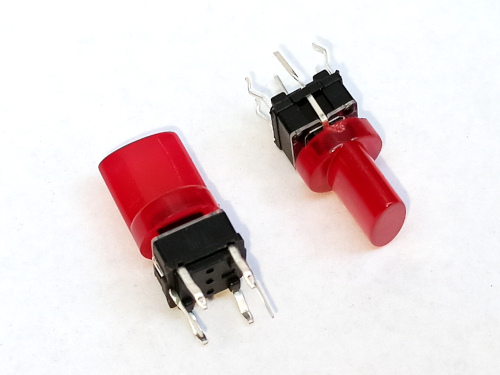
\includegraphics[scale=0.5]{assets/zekit-tacts-resized.jpg}
\end{center}

The tactile switches are momentary switches used as buttons. They feature a contact that is normally open and gets closed when the switch is pressed. The model of switch used in this kit has an additional LED that illuminates the cap to show status information. They are connected to the microcontroller directly.

\subsubsection{Toggle Switches}

\begin{center}
    (Todo: image)
\end{center}

In contrast to the tactile switches, the toggle switches have two stable positions. Depending on the position one contact is permanently closed while the other is open and vice versa. In the \textbf{zekit} these switches are used in the analog filter to select the mode (low-pass or band-pass) and resonance.

\subsubsection{Potentiometers}

\begin{center}
    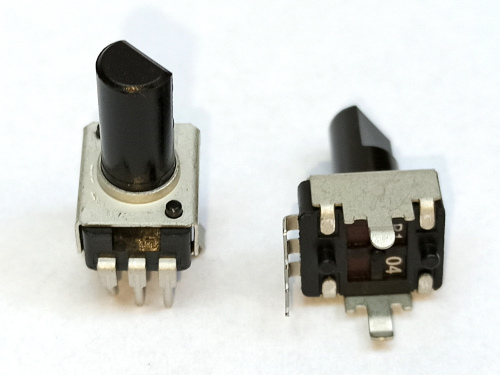
\includegraphics[scale=0.5]{assets/zekit-pots1-resized.jpg}
    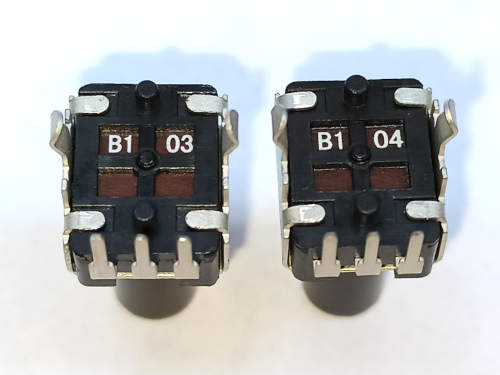
\includegraphics[scale=0.5]{assets/zekit-pots2-resized.jpg}
\end{center}

The potentiometers are variable resistors used to control parameters in the analog domain. They consist of a wiper that slides over a resistive element to form a voltage-divider.

The \textbf{zekit} uses two types of potentiometers with different values: 10k and 100k. These must not be confused and can be identified by the labeling on the bottom. The 10k pot is marked with a \textbf{B1 03} print, the 100k pot has a \textbf{B1 04} labeling.

\subsubsection{Trim Potentiometers}

\begin{center}
    (Todo: image)
\end{center}

The trimmers work like normal potentiometers but are intended for calibration purposes instead of regular use. They are much smaller the regular pots and need to be adjusted via a screwdriver.

(Todo: labeling 1k / 10k)

\subsubsection{Power Switch}

\begin{center}
    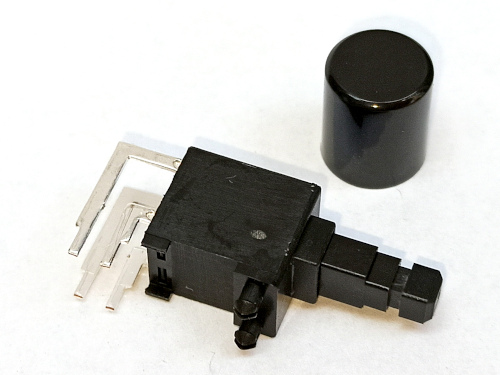
\includegraphics[scale=0.5]{assets/zekit-powerswitch-resized.jpg}
\end{center}

The power switch is a push button switch with a toggle behaviour. Pressed once, the contact closes and remains in this state until it is pushed again.

\subsubsection{Power Jack}

\begin{center}
    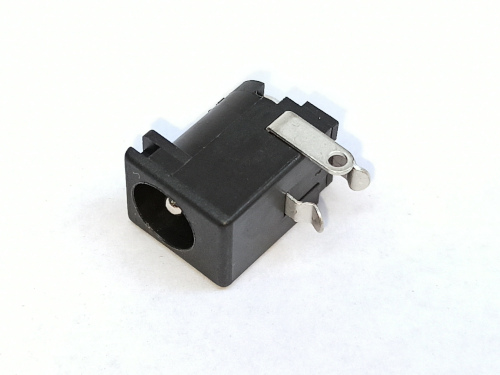
\includegraphics[scale=0.5]{assets/zekit-dcjack-resized.jpg}
\end{center}

The power jack is a barrel connector that has a widespread use with power supplies. It has an additional switch that is opened when a plug is inserted. This is useful in devices with internal batteries to disable them on external supply but not used in this kit.

\subsubsection{DIN Jack}

\begin{center}
    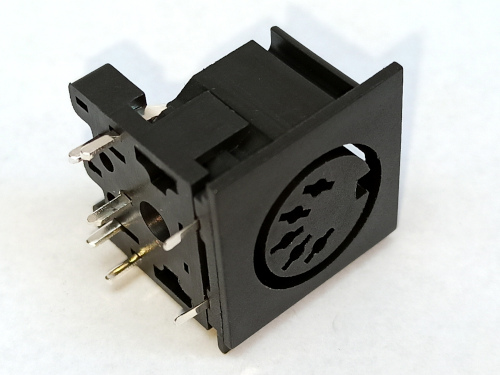
\includegraphics[scale=0.5]{assets/zekit-din-resized.jpg}
\end{center}

The DIN jack is a 5-pin connector that is used for the MIDI input from external devices.

\subsubsection{6.3mm TRS Jack}

\begin{center}
    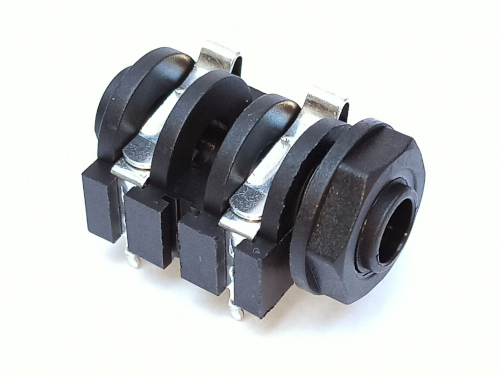
\includegraphics[scale=0.5]{assets/zekit-jack1-resized.jpg}
\end{center}

TRS stands for tip, ring, sleeve. This connector is common in all kinds of audio systems and used for the output signal of the \textbf{zekit}.

\subsubsection{3.5mm TRS Jacks}

\begin{center}
    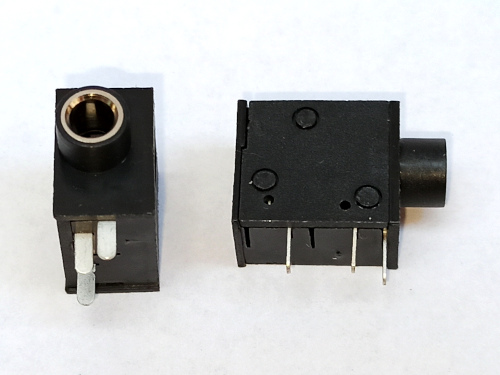
\includegraphics[scale=0.5]{assets/zekit-jack2-resized.jpg}
\end{center}

These jacks are the smaller versions of the TRS jack. In the \textbf{zekit}, they are used for the audio and clock inputs.

\subsubsection{Film Capacitors}

\begin{center}
    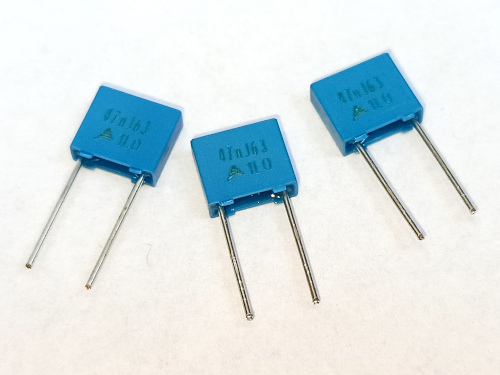
\includegraphics[scale=0.5]{assets/zekit-filmcaps-resized.jpg}
\end{center}

The film capacitors behave like normal capacitors but are superior in terms of distortion and noise immunity. They also have lower tolerances and are used in situations where these characteristics are important: in the \textbf{zekit} that's the filter and the VCA.

\subsubsection{Potentiometer Knobs}

\begin{center}
    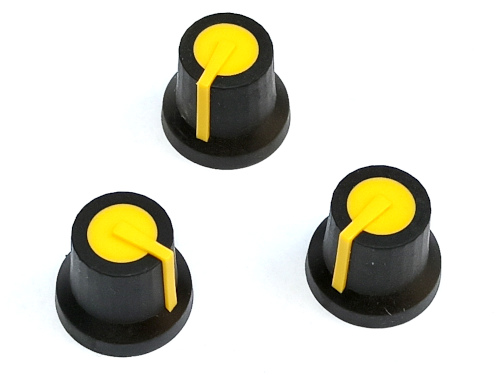
\includegraphics[scale=0.5]{assets/zekit-knobs-resized.jpg}
\end{center}

The knobs are fit onto the potentiometers after the kit is fully assembled. They provide the final look-and-feel and allow precise control of the potentiometer setting.

\subsubsection{Microcontroller IC}

\begin{center}
    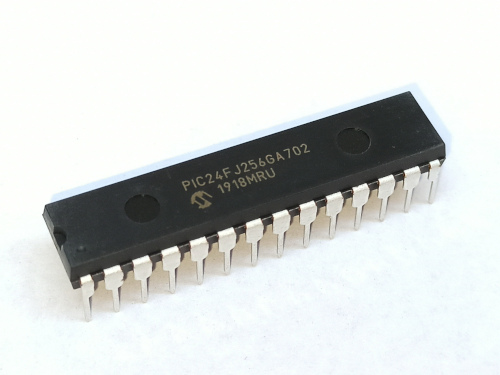
\includegraphics[scale=0.5]{assets/zekit-mcu-resized.jpg}
\end{center}

The microcontroller is an integrated circuit that contains flash memory to store the firmware, RAM for data and a number of peripherals to communicate with other components. It is used to calculate the audio waveforms, process incoming MIDI messages and clock signals, manage button presses and LEDs, and also to generate control signals for the envelopes.

The firmware to handle all these tasks is already pre-pregrammed by Fred’s Lab, but can be replaced by using a dedicated programmer kit.

\subsubsection{Optocoupler ICs}

\begin{center}
    (Todo: images)
\end{center}

An optocoupler is a combination of a photo transistor and an LED inside a single package. It is used keep circuits isolated while transferring signals. The conductance of the photo transistor is related to the brightness of the LED. The \textbf{zekit} uses optocouplers for the MIDI input and as variable resistors in the VCF and VCA.

\subsubsection{IC Sockets}

\begin{center}
    (Todo: correct image)
    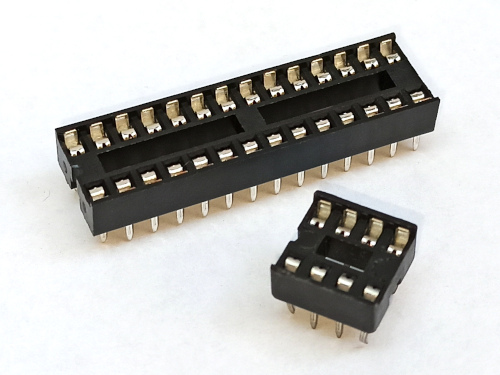
\includegraphics[scale=0.5]{assets/zekit-sockets-resized.jpg}
\end{center}

The IC sockets are mounted instead of soldering the ICs onto the PCB directly. They protect the ICs from the heat during the soldering process and keep them exchangeable.

\subsubsection{Enclosure Plates}

\begin{center}
    (Todo: image)
\end{center}

\pagebreak

% ------------------------------------------------------------------------------------------

\section{Assembling the Kit}

\subsection{General Advices}

\subsection{Setting Up the Soldering Gig}

\subsection{Soldering the Components}

It is advisable to solder the parts in a specific order which is mainly determined by the height of the components. Respecting the order can save you time and makes your life a lot easier.

Some useful tips:

\begin{itemize}
    \item Tape the components to prevent them from falling off when turning over the PCB for soldering
    \item All potentiometers and switches must be soldered straight. Otherwise, the front plate will not fit. To achieve this, solder only one pin first, then correct the position by gently pressing the part in the right position. After that, solder the remaining pins.
\end{itemize}

\vspace{0.25cm}

\begin{tcolorbox}
    \textcolor{red}{
        \textbf{Some components have a polarity and must be soldered in the right orientation. Even if they fit onto the PCB mechanically in more than one way, using the wrong orientation will result in erroneous operation and can even destroy these parts.}
    }
\end{tcolorbox}

\vspace{0.25cm}

\begin{tcolorbox}
    \textcolor{red}{
        \textbf{All connectors and the power switch are located on the bottom side of the PCB and must be soldered from the top.}
    }
\end{tcolorbox}

\subsubsection{IC Sockets}

The IC sockets have a marking on one side. This marking must match the silk screen print of the PCB.

\subsubsection{Film Capacitors}

These capacitors are more heat sensitive than other parts. Try to solder them quickly so that they are not exposed to the heat for a long time.

\subsubsection{1k Trimmer}

This trimmer is labeled \textbf{W102} on the top. Do not confuse it with the 10k variant.

\subsubsection{10k Trimmer}

This trimmer is labeled \textbf{W103}. Do not confuse it with the 1k variant.

\subsubsection{Tactile Switches}

While the switch itself works in all orientations, the internal LED must have the correct polarity. The pins of the LEDs have different lengths. The shorter pins must be located on the right side of the switch. (Todo: check / image).

Keep your attention on soldering them straight.

\subsubsection{Toggle Switches}

(Todo: write something useful). Keep your attention on soldering them straight.

\subsubsection{10k Potentiometers}

These 2 pots are labeled \textbf{10 B3} on the bottom. Do not confuse them with the 100k variants. Keep your attention on soldering them straight.

\subsubsection{100k Potentiometers}

These 4 pots are labeled \textbf{10 B4} on the bottom. Do not confuse them with the 10k variants. Keep your attention on soldering them straight.

\subsubsection{Connectors \& Power Switch}

The connectors and the power switch are soldered last because they are located on the bottom side of the PCB.

\subsection{Installing the ICs}

(Todo: maybe power up and measure supply voltages before)

\begin{itemize}
    \item MIDI optocoupler
    \item VCF/VCA Optocoupler
    \item Microcontroller
\end{itemize}

\section{Power Up and Test}

 (Todo: what to expect)

\subsection{Calibration of the VCF}

(Todo: adjusting the trimmers)

\subsection{Identifying Common Issues}

\begin{itemize}
    \item Bad soldering
    \item Wrong polarity (Todo: of what? ICs?)
\end{itemize}

\pagebreak

% ------------------------------------------------------------------------------------------

\section{Functional Description}

\subsection{Power Supply}

The Zekit needs the energy delivered by the power supply. This block provides 2 voltages: +3.3V and -2V, using a linear regulator and a charge pump respectively.

\subsubsection{Linear Regulator}

\begin{center}
    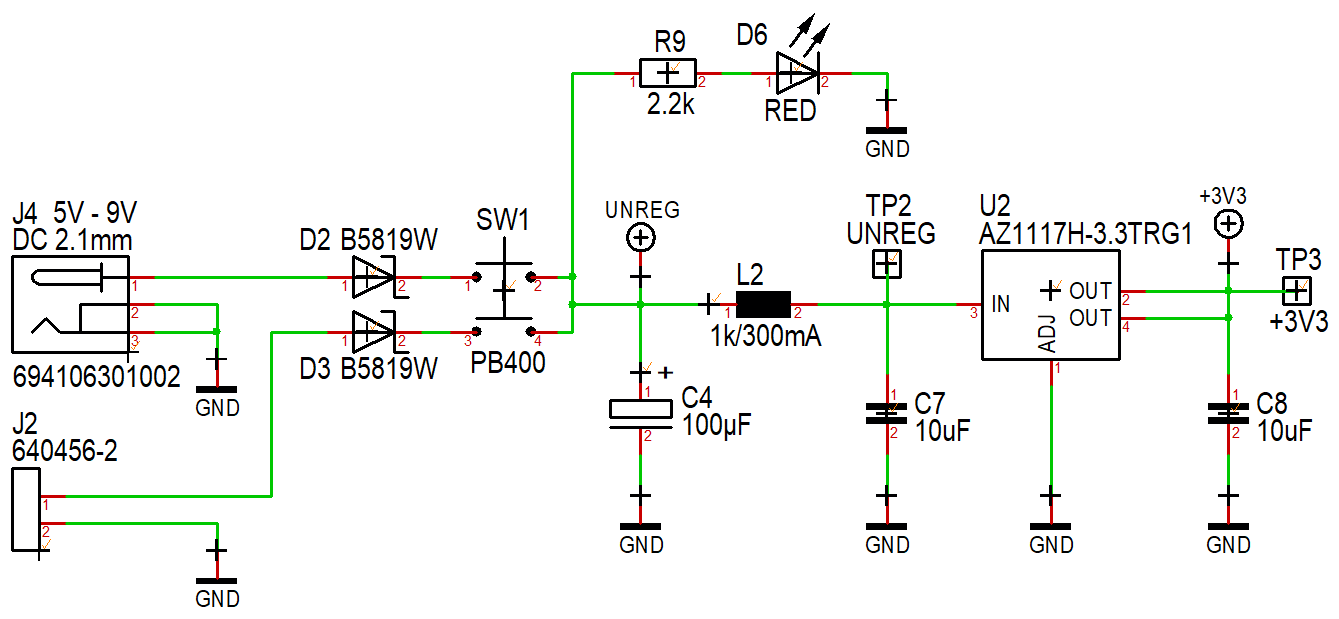
\includegraphics[scale=0.4]{assets/schema-power.png}
\end{center}

\emph{SW1} is the power switch. \emph{D3} ensure voltage polarity is correct, by letting the current flows only in the right direction. \emph{C4}, \emph{R9} \& \emph{C7} filter the input voltage, reducing supply noise. \emph{U2} regulates down the input, assuring a stable +3V3 in all circumstances. \emph{C8} secures \emph{U2} against possible oscillation of its output voltage.

\subsubsection{Charge Pump}

\begin{center}
    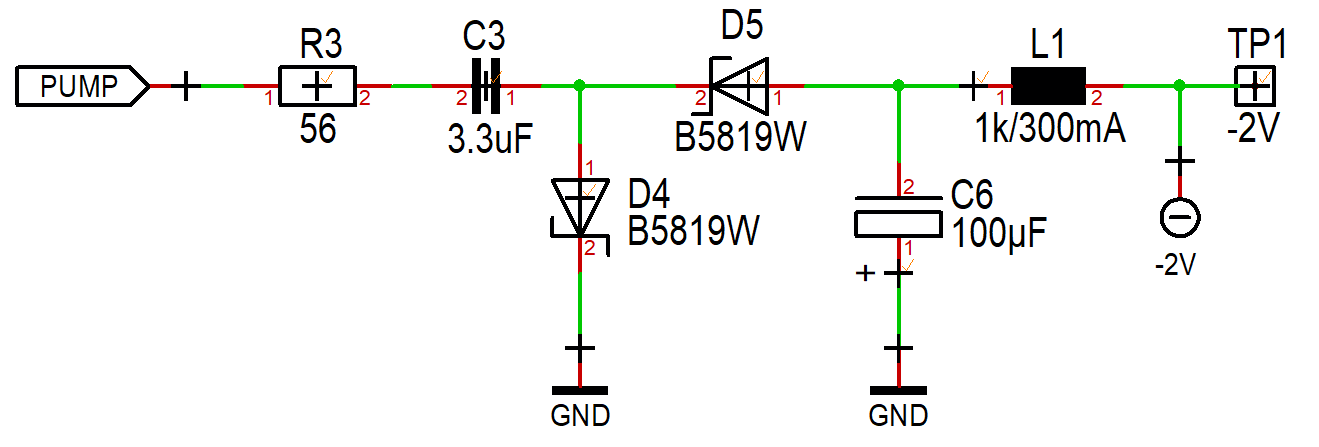
\includegraphics[scale=0.3]{assets/schema-pump.png}
\end{center}

The \emph{PUMP} signal is fed by the microcontroller and alternates between GND and +3.3V at a high frequency. When \emph{PUMP} is at +3.3V, \emph{C3} is charged via \emph{R3} and \emph{D2}, while \emph{D4} is non-conductive. When \emph{PUMP} is at GND, \emph{D2} is isolating and the charge of \emph{C3} is transferred to \emph{C5} via the now conducting \emph{D4}. The inductor \emph{L1} filters the voltage for better noise immunity.

Ideally, the output voltage at \emph{TP1} would be -3.3V, but because of the loss inside the diodes, it will be around -2V, which is still sufficient for proper operation.

\subsection{Microcontroller}

\begin{center}
    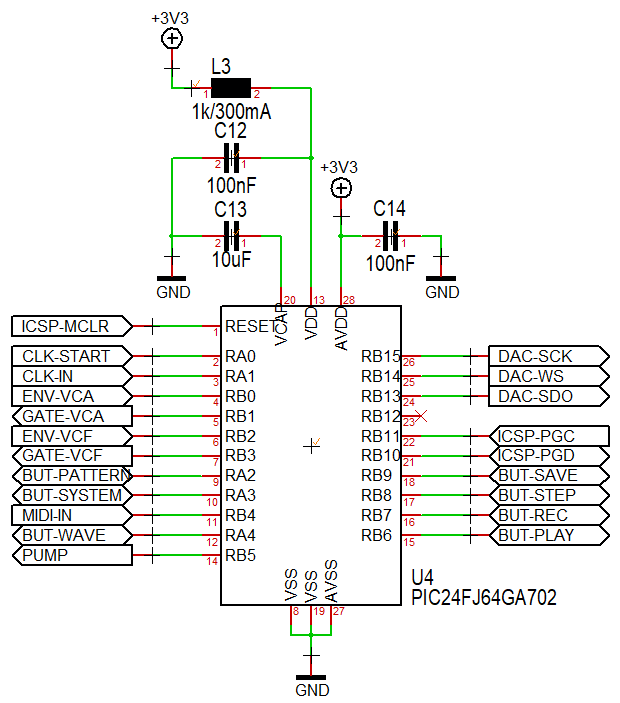
\includegraphics[scale=0.55]{assets/schema-mcu.png}
\end{center}

The microcontroller (MCU) \emph{U7} is the brain of the \textbf{zekit}. It processes all signals from the switches and the inputs and generates the audio waveform as well as some control signals for the analog circuitry. This is done by running a firmware that is stored in the internal flash of the chip.

The capacitors \emph{C11}, \emph{C12} and \emph{C14} are used together with the inductor \emph{L2} to improve the stability of the power supply and reduce noise.

\subsection{DAC}

\begin{center}
    (Todo: DAC schematics)
    % 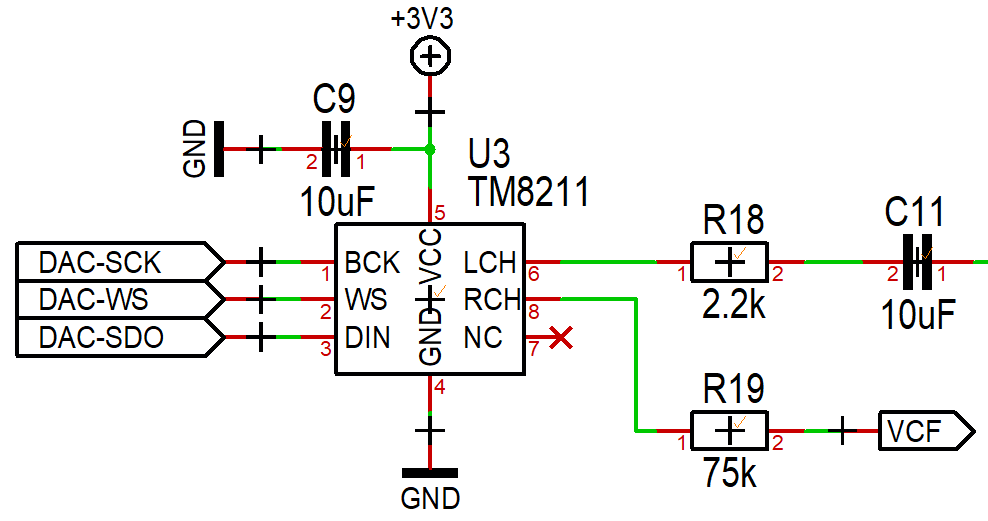
\includegraphics[scale=0.55]{assets/schema-dac.png}
\end{center}

The digital-to-analog converter (DAC) \emph{U3} is directly connected to the microcontroller via 3 signals. It converts the waveform calculated by the MCU into the analog domain. Capacitor \emph{C13} removes the DC offset of the signal, resistor \emph{R19} conditions the level to fit in the range of the next stage (the VCF).

The DAC chip provides two independent output channels of which only one is used internally. The unused channel is routed to the test point \emph{TP4} and can be utilized for additional purposes.

\subsection{VCF}

\begin{center}
    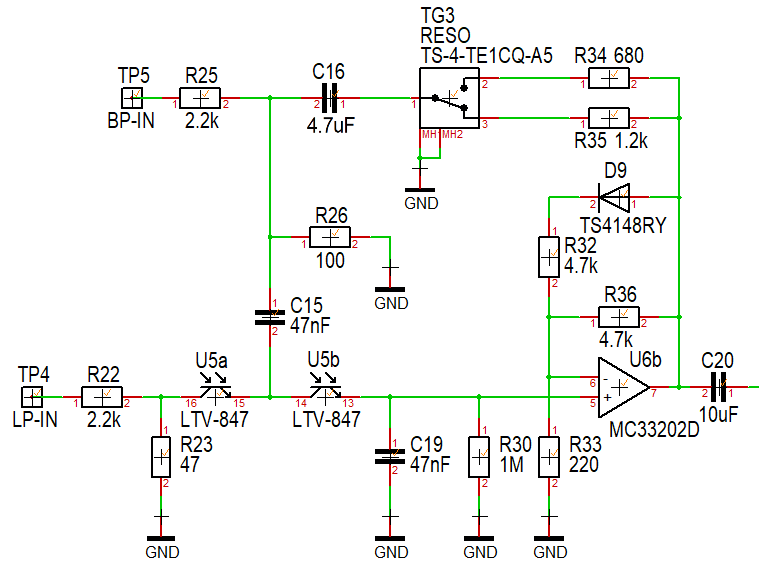
\includegraphics[scale=0.39]{assets/schema-vcf.png}
\end{center}

The filter is a 2nd order design with a 12dB/octave slope. The first stage consists of the optocoupler \emph{U3a/U3b} and the capacitor \emph{C15}, the second one of optocoupler \emph{U3b} and capacitor \emph{C19}, in which the optocouplers take the role of the resistive element to control the frequency.

The input signal \emph{VCF-IN} is decoupled by \emph{C13} and fed in either to the first stage or the feedback path, depending whether low-pass or band-pass configuration is selected by toggle switch \emph{TG1}. The resonance is determined by the feedback loop and can be chosen between two amounts via toggle switch \emph{TG2}. The trimmer \emph{TR2} allows to fine-control one of the settings. The operational amplifier \emph{U6b} provides the necessary gain for driving the next stage and the feedback loop. It utilizes the diode \emph{D7} to tame the amplitude at higher levels by producing a nice-sounding distortion.

\subsection{VCA}

\begin{center}
    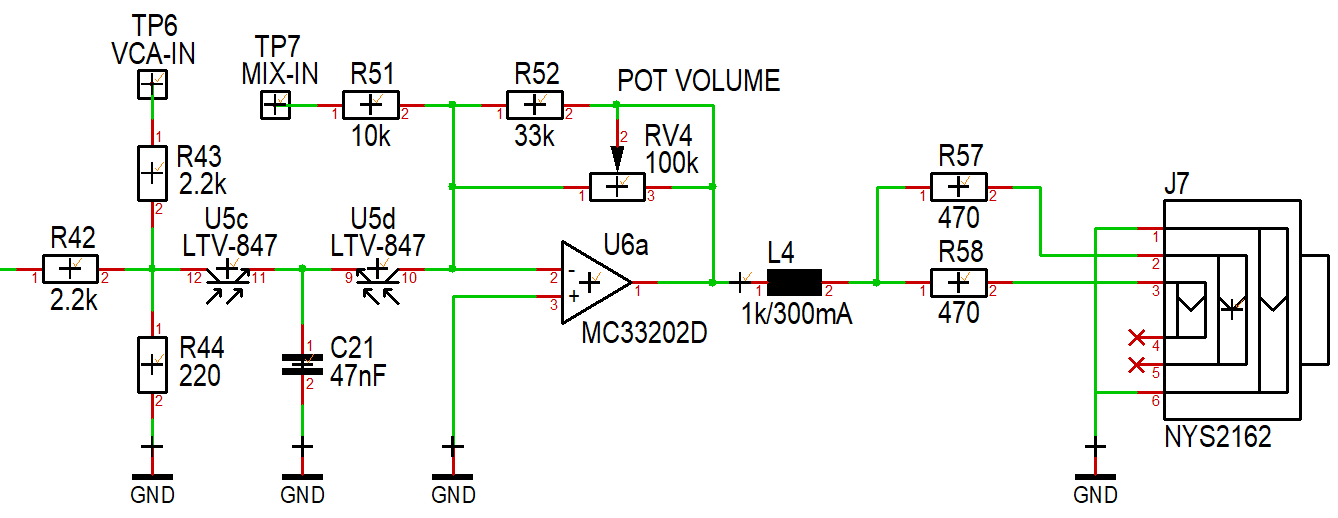
\includegraphics[scale=0.37]{assets/schema-vca.png}
\end{center}

The VCA uses the optocoupler \emph{U3c/U3d} to gain-control the operational amplifier \emph{U6a}. The input signal \emph{VCA-IN} is decoupled by capacitor \emph{C20} and then divided down by resistors \emph{R39} and \emph{R40} to an appropriate level for the optocoupler. To set the output level, the \textbf{Volume} potentiometer is located in the feedback path of the opamp. Resistor \emph{R47} in parallel to the pot provides a nicer control curve for the volume setting. The output is filtered by inductor \emph{L1}, followed by protection resistors \emph{R51} and \emph{R52} and then routed to the output jack \emph{J6}.

\subsection{Envelopes}

\subsubsection{VCF Envelope}

\begin{center}
    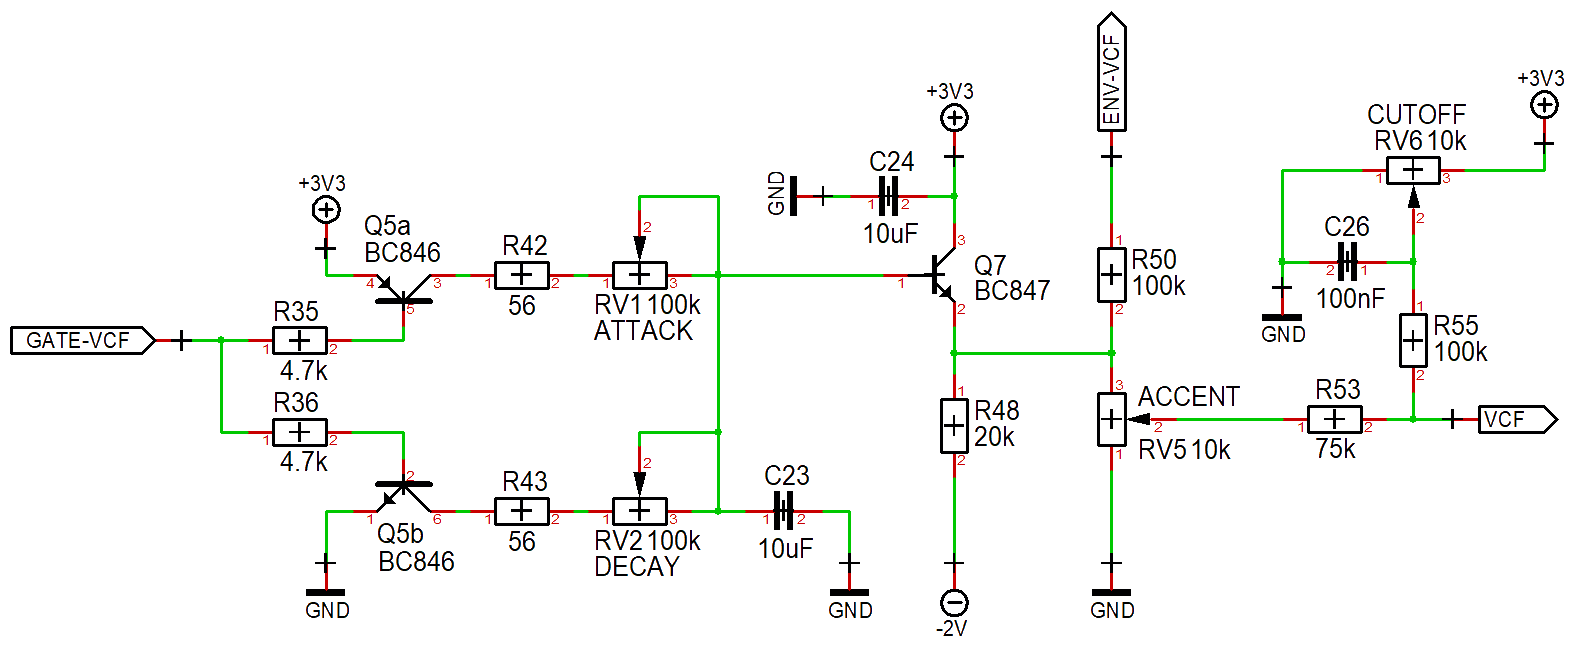
\includegraphics[scale=0.36]{assets/schema-ar.png}
\end{center}

The filter envelope is generated by either charging capacitor \emph{C23} to +3.3V or discharging it to GND. To start the envelope, the microcontroller sets the \emph{GATE-VCF} signal to +3.3V. The transistor \emph{Q5a} then conducts and \emph{C23} is charged via the resistor \emph{R42} and the \textbf{Attack} potentiometer. To put the envelope in release, the MCU sets the \emph{GATE-VCF} signal to GND. \emph{Q5a} then cuts off and \emph{Q5b} starts to conduct, resulting in \emph{C23} being discharged via \emph{R43} and the \textbf{Release} potentiometer.

The transistor \emph{Q7} acts as a buffer to decouple the envelope. The \emph{ENV-VCF} signal is routed back to the MCU so it can detect that the attack phase is finished. Finally, the envelope amount is set by the \textbf{Accent} potentiometer and added to the constant level set by the \textbf{Cutoff} potentiometer.

\subsubsection{VCA Envelope}

The amplifier envelope works in the same ways as the VCF envelope, but lacks the attack control.

\subsection{Exponential Control Circuit}

\begin{center}
    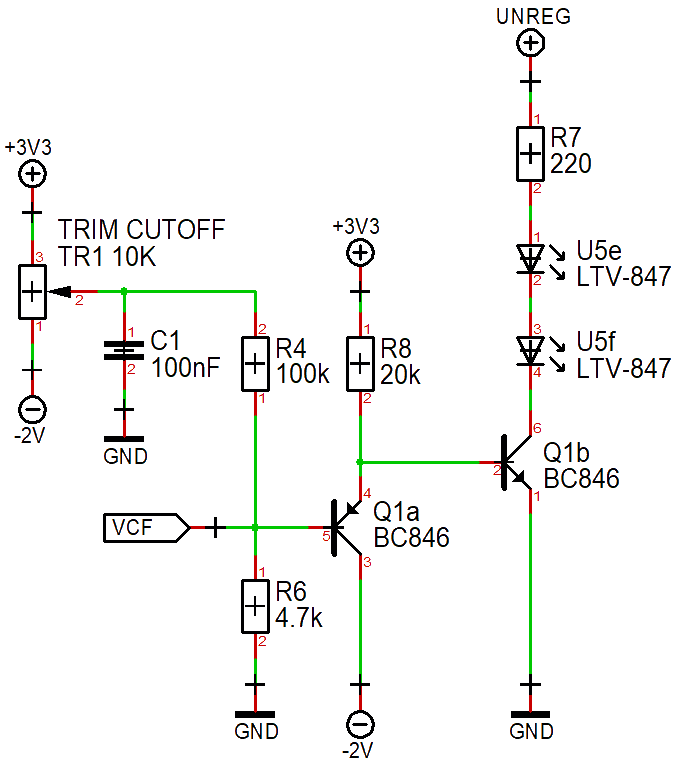
\includegraphics[scale=0.42]{assets/schema-expo.png}
\end{center}

This circuit is used to convert the linear control voltage into an exponential current for the optocouplers. The requirement for this is the nature of our human hearing which recognizes pitches and volumes in an exponential way.

The input of this block uses the signal \emph{VCF} from the filter envelope to drive the buffer transistor \emph{Q1a}. The trim potentiometer \emph{TR1} is used to set a bias level for calibration which is added to the input. The emitter of \emph{Q1a} drives the base of transistor \emph{Q1b} which does the curve conversion. It is based on the fact that the relationship between the base-emitter voltage and the collector current of a transistor is exponential. The collector current of \emph{Q1b} drives the LEDs inside the optocoupler \emph{U5} which controls the filter cutoff.

The VCA uses a similar circuit that is feeded by the VCA envelope.

\subsection{MIDI Input}

\begin{center}
    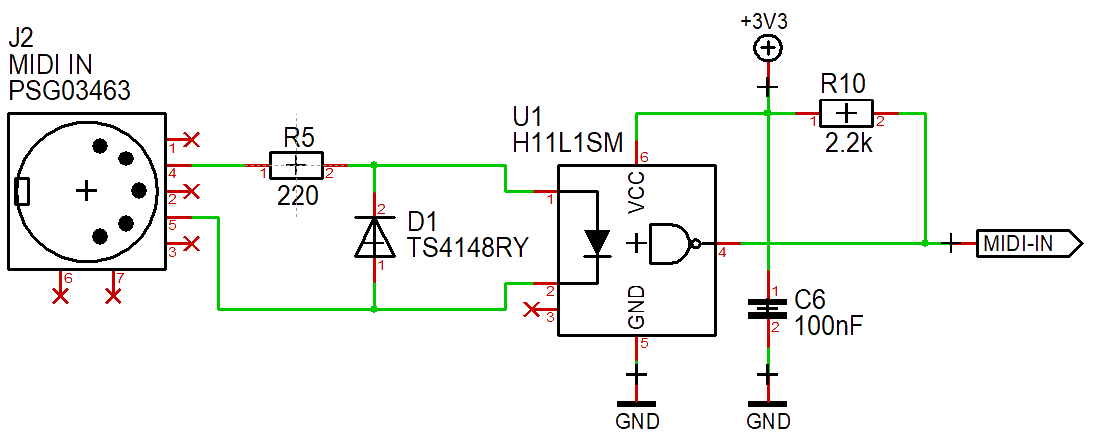
\includegraphics[scale=0.40]{assets/schema-midi.png}
\end{center}

The MIDI input is electrically isolated with an optocoupler to prevent ground loops. This is required by the official MIDI specification. The external device drives the LED inside the optocoupler \emph{U1} via the resistor \emph{R5}. When the LED is on, the photo transistor inside the optocoupler conducts and the \emph{MIDI-IN} signal is pulled to GND. When the LED is off, the photo transistor cuts off and \emph{MIDI-IN} is set to +3.3V by the pullup resistor \emph{R10}.

\subsection{Clock Input}

\begin{center}
    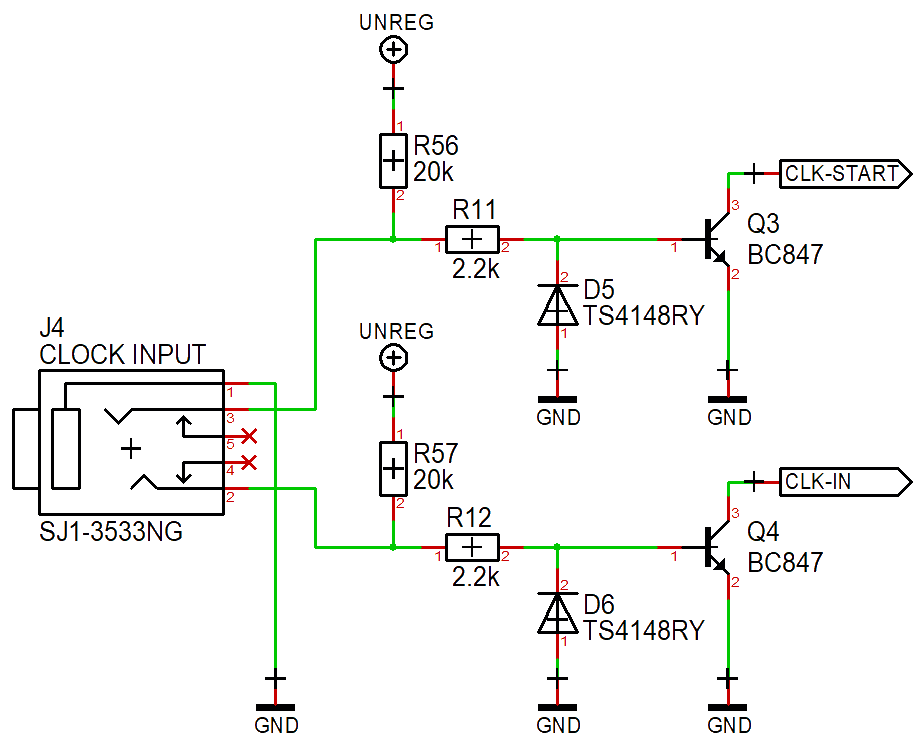
\includegraphics[scale=0.40]{assets/schema-clocks.png}
\end{center}

The clock signal is taken from the tip of the input jack \emph{J4}. If no plug is inserted, a high level is preset by the pullup resistor \emph{R57}. Depending on the input voltage, transistor \emph{Q4} is either conducting or not. Resistor \emph{R12} and diode \emph{D6} protect the transistor against over-voltage or wrong polarity at the input. At the end, the signal \emph{CLK-IN} is then routed to the microcontroller. The MCU uses an internal pullup activated by the firmware to detect the high level when transistor \emph{Q4} is off.

The clock start signal is taken from the ring of the input jack and processed in a similar way by driving the transistor \emph{Q3} to generate the \emph{CLK-START} signal for the MCU.

\subsection{Tactile Switches}

\begin{center}
    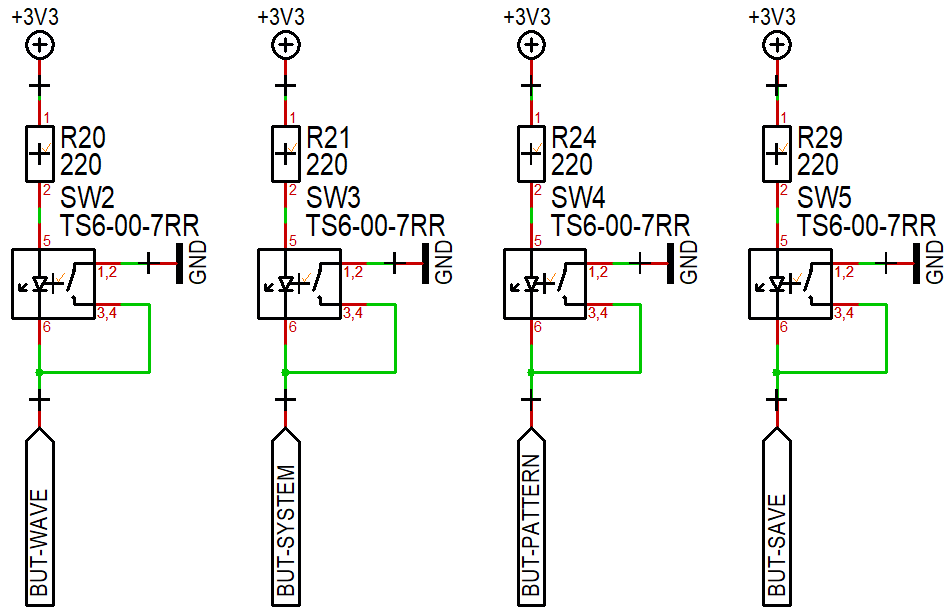
\includegraphics[scale=0.25]{assets/schema-switch.png}
\end{center}

The 7 illuminated tactile switches are directly connected to the microcontroller. The image above shows the \emph{WAVE} button switch \emph{SW2} as an example.

In order to reduce the number of required signal lines, the MCU firmware uses a neat trick: it alternates the mode of the pin connected to the \emph{BUT-WAVE} signal between input and output.

When the MCU pin is configured as input, the button state can be read. In case the button is released, a high level is detected because the pin is connected to +3.3V via the LED and the resistor \emph{R18}. When the button is pressed, the pin is directly connected to GND and a low level is detected. When the MCU pin is configured as output, the LED can be illuminated by driving the signal to GND.

\pagebreak

% ------------------------------------------------------------------------------------------

\section{Additional Resources}

=> The github
=> The webpage
=> Where to find the MCU source code

\pagebreak

% ------------------------------------------------------------------------------------------

\section{Legal / License}

\pagebreak

% ------------------------------------------------------------------------------------------

\section{Operation}

 (Todo: user manual)

% ------------------------------------------------------------------------------------------

\section{Schematics}

To minimize electronic waste and ensure long product life, Fred’s Lab is willing to provide all technical documents needed to repair his products. The following schematics are provided ”as is” with no warranty of any kind. Any modification made to a Fred’s Lab instrument immediately voids the included 3-year product warranty. Repairs must be carried out by a competent repair service. Fred’s Lab stays available for the maintenance of your instruments. Do not hesitate to contact the support service for a free quote. Spare parts can directly be ordered from us.

\textbf{Intellectual property:}

The following technical documents are provided for advisory, repair and educational purposes only. They remain the entire property of Fred's Lab and cannot be reproduced without a written authorization. Users are granted to draw inspiration from this information for their projects (commercial or not), while respecting the limits of non-cloning or counterfeiting the original product. If in doubt about legal matters, please contact us.

\begin{center}
    (Todo: full schematics)
    % 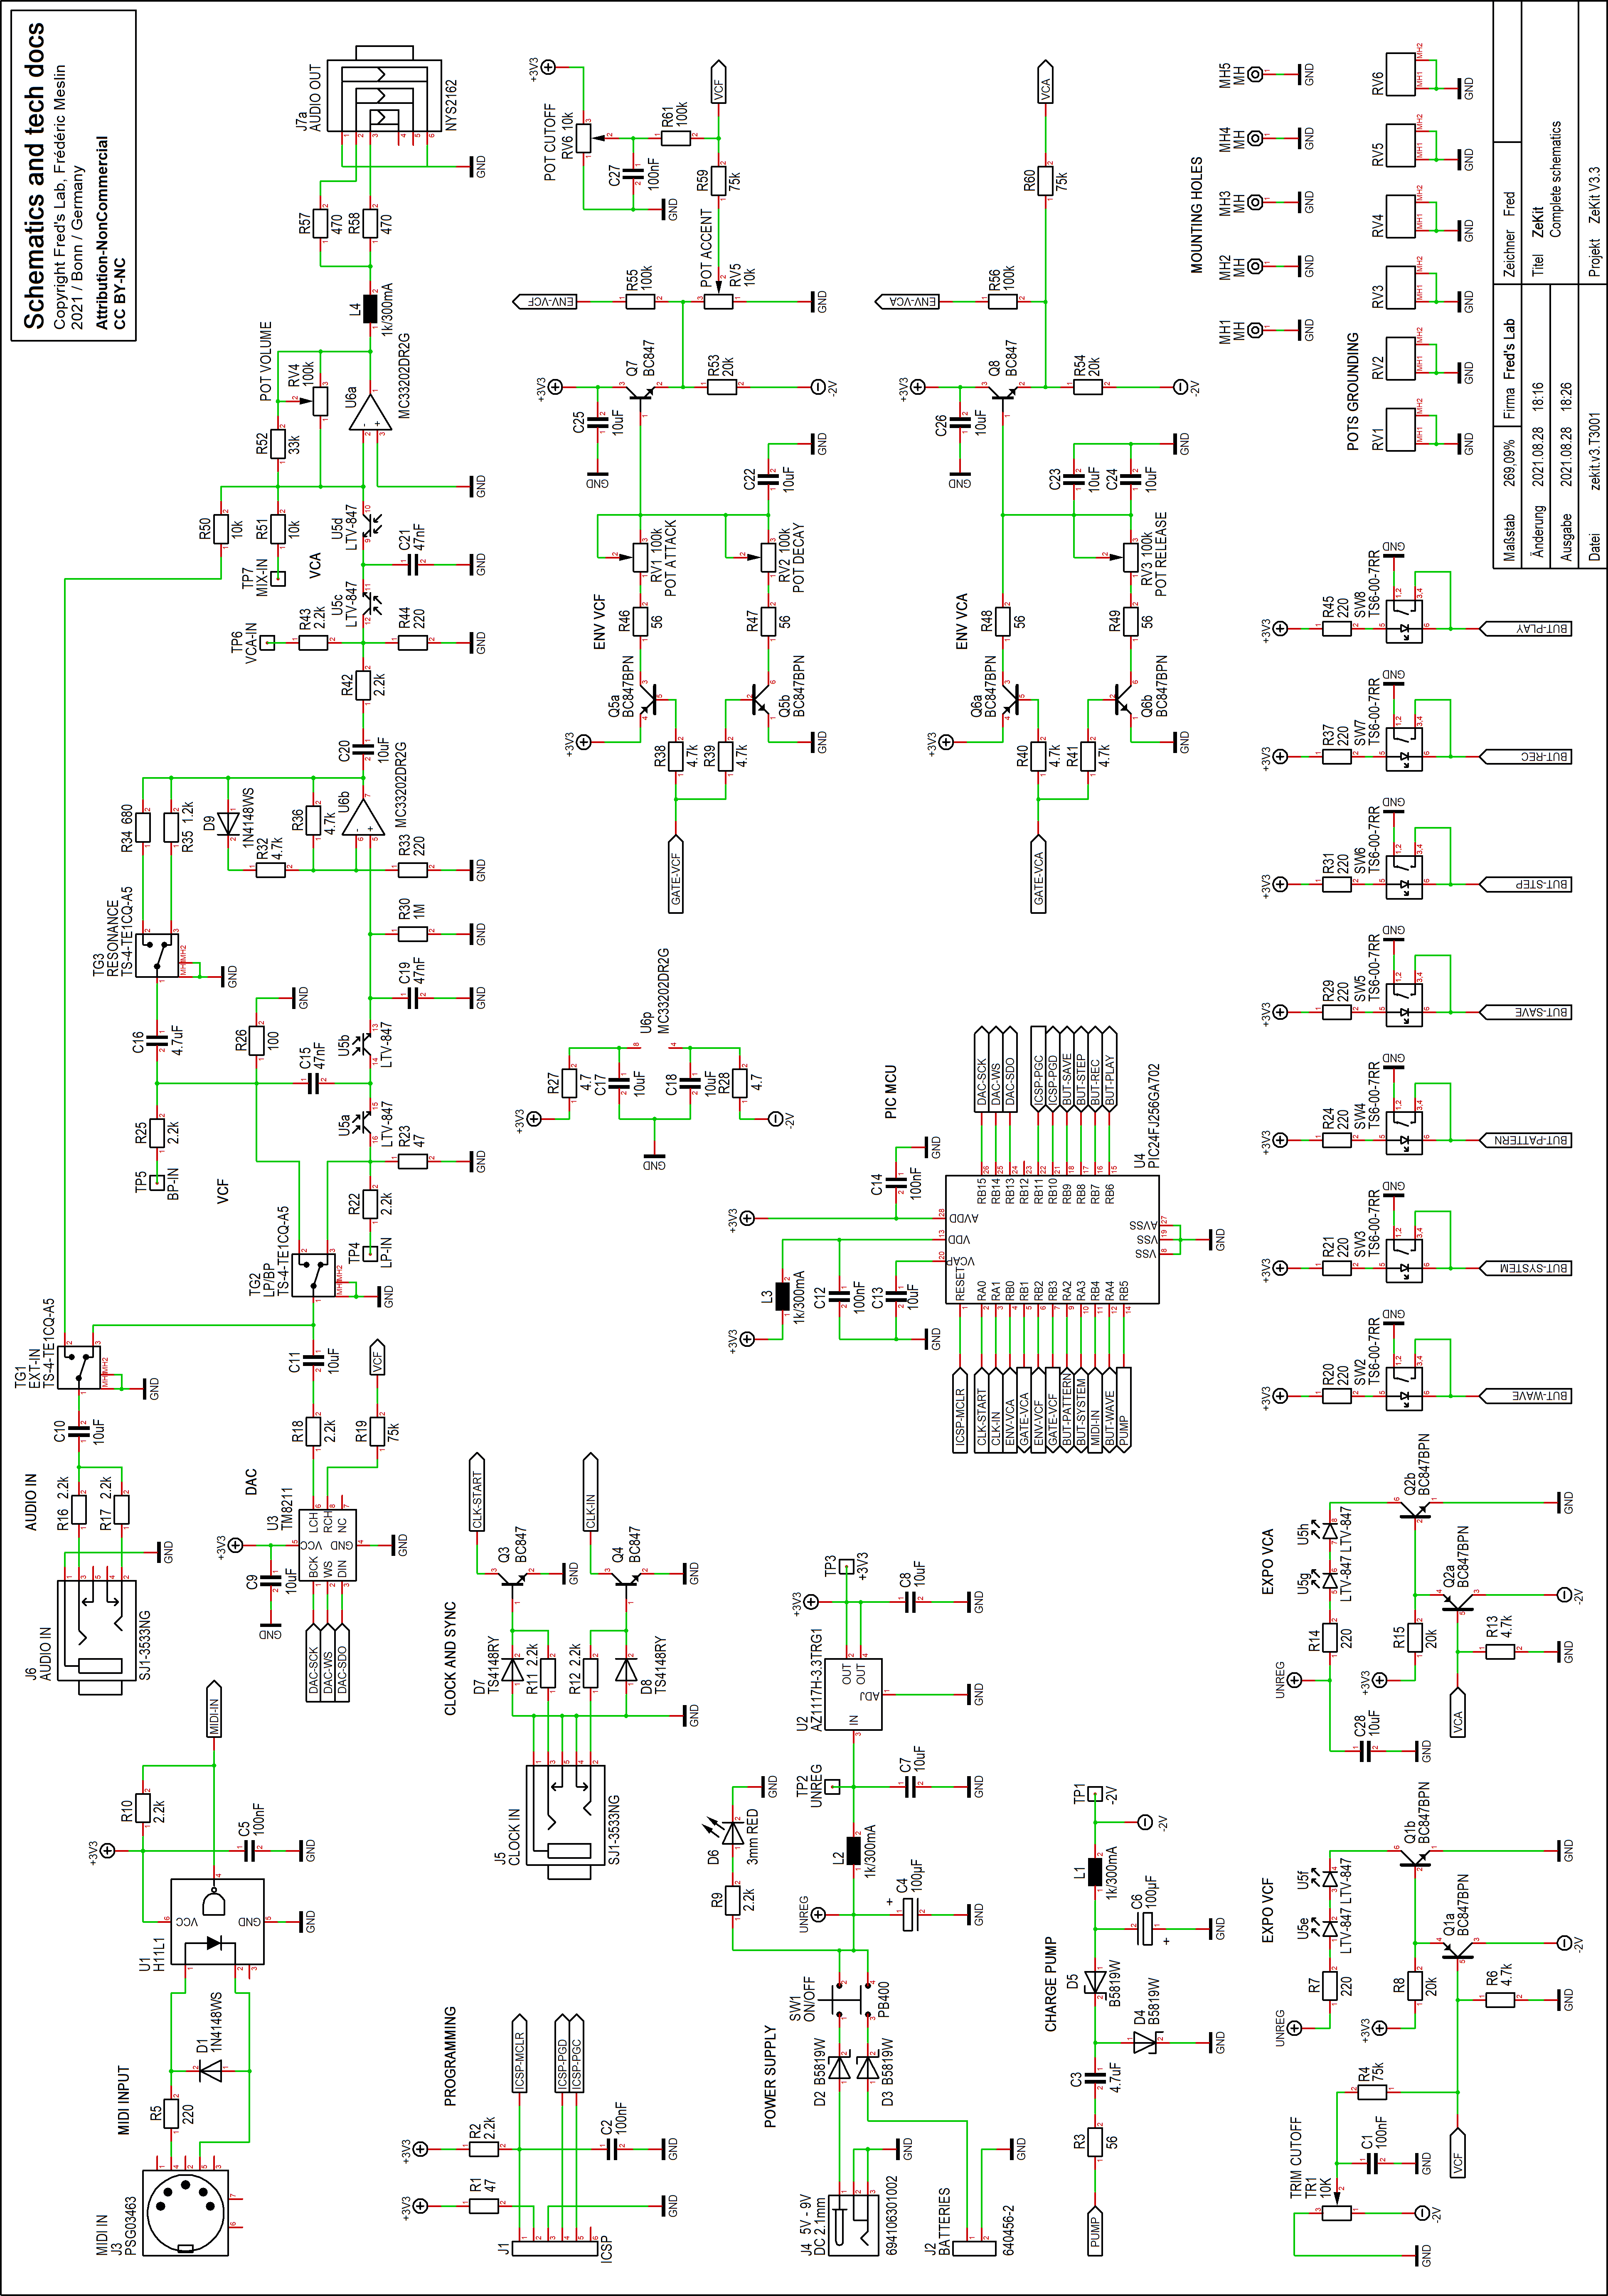
\includegraphics[scale=0.7,angle=90,origin=c]{assets/schema-full.png}
\end{center}


\end{document}
